% !TEX TS-program = lualatex
%\batchmode

\documentclass[professionalfonts,aspectratio=169]{beamer}
\usetheme[subsectionpage=progressbar]{metropolis}

\usefonttheme[onlymath]{serif}
\newfontfamily\sfamily{STIX Two Text}
\usepackage{mathtools,amssymb}

\usepackage{unicode-math}
\setmathfont{STIX Two Math}
\usepackage{microtype}
\usepackage{lualatex-math}

%\usepackage[italian,english]{babel}
\usepackage{polyglossia}
\setdefaultlanguage[variant=british]{english}
\setotherlanguage{italian}
\usepackage{csquotes}


% Adjoint
\newcommand{\adj}[1]{\overline{#1}}
% Average
\newcommand{\average}[1]{\overline{#1}}
% Trace operator
\DeclareMathOperator{\tr}{Tr}
% Differential operator
\DeclareMathOperator{\D}{d}

\usepackage{slashed}
\usepackage{tensor}

% Enhanced tabs
\usepackage{booktabs,caption}

\usepackage{mdframed}

\begin{document}

\author{Relatore: Dott.ssa Fulvia De Fazio \\ Laureando: Stefano Campanella}
\title{Spectroscopy of Charmed Hadrons}
\subtitle{Facing the Latest Experimental Results with the Theory}
\date{April 26, 2018}
\institute{Università degli Studi di Bari}

\maketitle

\section{Presentation Outline}

\begin{frame}{My thesis in brief}

  The core of my thesis consisted in the calculations, within the framework
  of heavy chiral perturbation theory, of branching fraction ratios
  of a recently observed excited $D$ meson, the $\left. D \right.^*_2(3000)$, 
  aimed at its classification.

\end{frame}

\begin{frame}{Structure of the presentation}
  \begin{enumerate}
    \item \textbf{Why?} → Recent experimental findings in hadron spectroscopy.
      \pause
    \item \textbf{How?} → The theoretical framework: an effective field theory approach.
      \pause
    \item \textbf{What are the implications?} → Classification of the charmed mesons.
      \pause
    \item \textbf{What’s the point?} → Identification of the $D^*_2(3000)$.
      \pause
    \item \textbf{So What?} → Conclusions and perspectives.
  \end{enumerate}
\end{frame}

\section{Advances in Hadron Spectroscopy}

\begin{frame}{Bird-eye view}
  \pause
  \begin{block}{Exotic spectroscopy}
    \vspace{0pt}
    \begin{itemize}
    \item Supernumerary states (es. $X(3872)$, $Y(4260)$, \ldots{}).
    \item Charged quarkoniumlike states (es. $Z(4430)^+$, 
      $Z(4200)^+$, \ldots{}).
    \item Pentaquark states ($P_c(4380)^+$, $P_c(4450)^+$).
  \end{itemize}
\end{block}
\pause
\begin{block}{Ordinary spectroscopy}
  \vspace{0pt}
  \begin{itemize}
  \item Heavy baryons
  \item Heavy mesons ← \emph{The subject of my thesis!}
\end{itemize}
  \end{block}
\end{frame}

\subsection{Charmed Mesons: Latest Observations}

\begin{frame}
  Leading role: $B$-factories (Belle, BaBar), LHCb
  
  Latest observations: \\ 2010 (BaBar), 2013 (LHCb) 
  and \textbf{2016 (LHCb)} ← \alert{Observation of the $D^*_2(3000)$!}

  \begin{columns}
    \captionsetup{skip=1pt}
    \begin{column}{0.5\textwidth}
      \begin{table}
        \fontsize{4.5pt}{6pt}\selectfont
        \centering
        \begin{tabular}{*{4}{@{\hskip 2pt}c@{\hskip 2pt}}}
          \toprule
          Resonance & mass (MeV) & $\Gamma$ (MeV) & $J^P$ \\ 
          \midrule
          $D(2550)^0 $ & $2539.4 \pm 4.5 \pm 6.8$ & $130 \pm 12 \pm 13$ & $0^-$ \\
          \addlinespace[2pt]
          $D^*(2600)^0$ & $2608.7 \pm 2.4 \pm 2.5$ & $93 \pm 6 \pm 13$ & natural \\
          $D^*(2600)^\pm$ & $2621.3 \pm 3.7 \pm 4.2$ & $93 \ \text{(fixed)}$ & natural \\
          \addlinespace[2pt]
          $D(2750)^0$ & $2752.4 \pm 1.7 \pm 2.7$ & $71 \pm 6 \pm 11$ & \\
          \addlinespace[2pt]
          $D^*(2760)^0$ & $2763.3 \pm 2.3 \pm 2.3$ & $60.9  \pm 5.1 \pm 3.6$ & natural \\
          $D^*(2760)^\pm$ & $2769.7 \pm 3.8 \pm 1.5$ & $60.9 \ \text{(fixed)}$ & natural \\
          \bottomrule
        \end{tabular}
        \caption*{\tiny BaBar (2010)}
      \end{table}
      \vspace*{-\baselineskip}
      \begin{table}
        \fontsize{4.5pt}{6pt}\selectfont
        \centering
        \begin{tabular}{*{4}{@{\hskip 2pt}c@{\hskip 2pt}}}
          \toprule
          Resonance & mass (MeV) & $\Gamma$ (MeV) & $J^P$ \\ 
          \midrule
          $D^*_1(2680)^0$   & $2681.1 \pm 5.6 \pm 4.9 \pm 13.1$ & $186.7 \pm 8.5 \pm 8.6 \pm 8.2$  & $1^-$ \\
          $D^*_3(2760)^0$   & $2775.5 \pm 4.5 \pm 4.5 \pm 4.7$  & $95.3  \pm 9.6 \pm 7.9 \pm 33.1$ & $3^-$ \\
          \alert{$D^*_2(3000)^0$}   & $3214   \pm 29  \pm 33  \pm 36$   & $186   \pm 39  \pm 34  \pm 63$   & $2^+$ \\
          \bottomrule
        \end{tabular}
        \caption*{\tiny LHCb (2016)}
      \end{table}
      \vspace*{-3\baselineskip}
    \end{column}
    \begin{column}{0.5\textwidth}
      \begin{table}
        \fontsize{4.5pt}{6pt}\selectfont
        \centering
        \begin{tabular}{*{4}{@{\hskip 2pt}c@{\hskip 2pt}}}
          \toprule
          Resonance & mass (MeV) & $\Gamma$ (MeV) & $J^P$ \\ 
          \midrule
          $D_J(2580)^0$     & $2579.5 \pm 3.4 \pm 5.5$  & $177.5 \pm 17.7 \pm 46.0$ & unnatural \\
          \addlinespace[2pt]
          $D^*_J(2650)^0$   & $2649.2 \pm 3.5 \pm 3.5$  & $140.2 \pm 17.1 \pm 18.6$ & natural \\
          \addlinespace[2pt]
          $D_J(2740)^0$     & $2737.0 \pm 3.5 \pm 11.2$ & $73.2 \pm 13.4 \pm 25.0$  & unnatural \\
          \addlinespace[2pt]
          $D^*_J(2760)^0$   & $2761.1 \pm 5.1 \pm 6.5$  & $74.4 \pm 4.3 \pm 37.0$   & natural \\
          $D^*_J(2760)^0$   & $2760.1 \pm 1.1 \pm 3.7$  & $74.4 \pm 3.4 \pm 19.1$   & natural \\
          $D^*_J(2760)^\pm$ & $2771.7 \pm 1.7 \pm 3.8$  & $66.7 \pm 6.6 \pm 10.5$   & natural \\
          \addlinespace[2pt]
          $D_J(3000)^0$     & $2971.8 \pm 8.7$          & $188.1 \pm 44.8$          & unnatural \\
          \addlinespace[2pt]
          $D^*_J(3000)^0$   & $3008.1 \pm 4.0$          & $110.5 \pm 11.5$          & natural \\
          $D^*_J(3000)^\pm$ & $3008.1 \ \text{(fixed)}$ & $110.5 \ \text{(fixed)}$  & natural \\
          \bottomrule
        \end{tabular}
        \caption*{\tiny LHCb (2013)}
      \end{table}
      \vspace*{-3\baselineskip}
    \end{column}
  \end{columns}
\end{frame}

%\begin{frame}
%  $B$-decay studies fix both spin and parity.
%
%  Prompt production studies fix only spin-parity series:
%  \begin{itemize}
%    \item natural ($0^+,\ 1^-,\ 2^+, \ldots{}$)
%    \item unnatural ($0^-,\ 1^+,\ 2^-, \ldots{}$)
%  \end{itemize}
%\end{frame}




\section{The Theoretical Framework}

\begin{frame}
  It is unclear how to describe analytically relativistic bound systems in quantum field theories.
  \pause

  The approaches used in hadron spectroscopy so far:
  \begin{enumerate}
    \item Potential models (i.e.~Schroedinger eq. with \emph{ad hoc} potentials)
    \item QCD effective theories ← \emph{The one used in my thesis!}
  \end{enumerate}
  \pause
  
  Effective theories leverage symmetries emerging from QCD in well defined limits.
\end{frame}

\subsection{Heavy Quark Symmetries}

\begin{frame}{Heavy quarks}
  Quarks within hadrons exchange gluons with $p \approx \Lambda_\text{\sfamily QCD} = 200 \, \text{\sfamily MeV} \approx 1 \, \text{\sfamily fm}^{-1}$.

  Quarks with $m_Q \gg \Lambda_\text{\sfamily QCD}$ 
  referred to as heavy ($c$, $b$). ← \alert{$t$ bound states unobserved!}
\end{frame}

\begin{frame}{Heavy Quark Effective Theory (HQET)}
  QCD Lagrangian for Heavy Quarks (HQ)
  \begin{equation*}
    \symcal{L}_\text{\sfamily QCD} = \adj{Q} \left( i \slashed{D} - m_Q \right) Q \qquad D_\mu = \partial_\mu - i g A^a_\mu T^a  \qquad \text{$Q$: HQ field}
  \end{equation*}
 
  \begin{block}{HQ limit $m_Q \to \infty$}
%    \footnotesize
%    \begin{equation*}
%      h(x) = e^{i m_Q v_\mu x^\mu} \frac{1 + \slashed{v}}{2} Q(x) \ , \qquad H(x) = e^{i m_Q v_\mu x^\mu} \frac{1 - \slashed{v}}{2} Q(x) % \\[10pt]
%    \end{equation*}
%    \normalsize
%
%    When $m_Q \to \infty$ (HQ limit), using the equations of motion
%    \footnotesize
    \begin{gather*}
      \symcal{L}_{\text{\sfamily QCD}} = \adj{h}_v \left. i v^\mu D_\mu \right. h_v + \frac{1}{2 m_Q} \adj{h}_v (i D_\perp)^2 h_v + \frac{g}{4 m_Q} \adj{h}_v \sigma_{\alpha \beta} G^{\alpha \beta} h_v + \symcal{O}\left( \frac{1}{m_Q^2} \right) \\
      h_v(x) = e^{i m_Q v_\mu x^\mu} \frac{1 + \slashed{v}}{2} Q(x) \qquad \text{← positive energy component of $Q$}%\ , \qquad H(x) = e^{i m_Q v_\mu x^\mu} \frac{1 - \slashed{v}}{2} Q(x)
    \end{gather*}
%    \normalsize
  \end{block}
 
  \begin{alertblock}{The HQET Lagrangian}
    \begin{equation*}
      \symcal{L}_\text{\sfamily HQET} \equiv \adj{h}_v \left. i v^\mu D_\mu \right. h_v
    \end{equation*}
  \end{alertblock}
\end{frame}

\begin{frame}[standout]
  In heavy hadrons the heavy quark decouples: \\
  HQ spin and flavour symmetries.
\end{frame}

\begin{frame}{Analogy with non-relativistic electrodynamics}
  There is an analogy with atomic spectroscopy (HQ ↔ nuclei):
  \begin{itemize}
    \pause
    \item HQ spin decoupling → hyperfine splitting is small
    \pause
    \item HQ flavour irrelevant → different isotopes have
    the same chemistry
  \end{itemize}
\end{frame}

\begin{frame}{Consequences of the HQ symmetries}
  For heavy mesons, in the exact HQ limit
  \begin{itemize}
    \pause
    \item
      Properties of beauty mesons related to those of charmed ones.
    \pause
    \item
      Mesons differing only for the orientation of the heavy quark spin expected to be degenerate.
    \pause
    \item
      Heavy quark spin $\vec{S}_Q$ and total angular momentum of the light degrees of freedom $\vec{S}_\ell$ separately conserved.
%    \pause
%    \item
%      Heavy meson states identified by
%      \begin{description}
%        \item{Heavy DOF}: \(\vec{S}_Q\), flavour (\(c\), \(b\))
%        \item{Light DOF}: \(n\), \(\vec{S}_q\), \(\vec{L}\), flavour (\(u\), \(d\), \(s\))
%      \end{description}
  \end{itemize}
\end{frame}


%\begin{frame}{HQET doublets}
%  \scriptsize
%  \begin{align*}
%    H =&  \frac{1 + \slashed{v}}{2} \left( \left. P^* \right._\mu \gamma^\mu - P \gamma^5 \right) \\[10pt]
%    S =& \frac{1 + \slashed{v}}{2} \left( \left. P^\prime_1 \right._\mu \gamma^\mu \gamma^5 - P^*_0 \right) \\
%    T^\mu =& \frac{1+\slashed{v}}{2} \left( \left. P^*_2 \right.\indices{^\mu_\nu} \gamma^\nu - \left. P_1 \right._\nu \sqrt{\frac{3}{2}} \gamma^5 \left( \eta^{\mu \nu} - \frac{1}{3} \gamma^\nu \left( \gamma^\mu - v^\mu \right) \right) \right) \\[10pt]
%    X^\mu =& \frac{1+\slashed{v}}{2} \left( \left. P_2 \right.\indices{^\mu_\nu} \gamma^\nu \gamma^5 - \left. P^{* \prime}_1 \right._\nu \sqrt{\frac{3}{2}} \left( \eta^{\mu \nu} - \frac{1}{3} \gamma^\nu \left( \gamma^\mu + v^\mu \right) \right) \right) \\
%    X^{\prime \mu \nu} =& \frac{1 + \slashed{v}}{2} \left( \left. P^*_3 \right.\indices{^{\mu \nu}_\rho} \gamma^\rho - \left. P^\prime_2 \right. \indices{_{\alpha \beta}} \sqrt{\frac{5}{3}} \gamma^5 \left( \eta^{\mu \alpha} \eta^{\nu \beta} - \frac{1}{5} \gamma^\alpha \eta^{\nu \beta} \left( \gamma^\mu - v^\mu \right) \right. \right. \nonumber \\
%    \phantom{X^{\prime \mu \nu} =}& \left. \left. - \frac{1}{5} \gamma^\beta \eta^{\mu \alpha} \left( \gamma^\nu - v^\nu \right) \right) \vphantom{\sqrt{\frac{5}{3}}} \! \right) , \\[10pt]
%    F^{\mu \nu} =& \frac{1 + \slashed{v}}{2} \left( \left. P_3 \right.\indices{^{\mu \nu}_\rho} \gamma^\rho \gamma^5 - \left. P^{* \prime}_2 \right.\indices{_{\alpha \beta}} \sqrt{\frac{5}{3}} \left( \eta^{\mu \alpha} \eta^{\nu \beta} - \frac{1}{5} \gamma^\alpha \eta^{\nu \beta} \left( \gamma^\mu + v^\mu \right) \right. \right. \nonumber \\
%  \phantom{F^{\mu \nu} =}& \left. \left. - \frac{1}{5} \gamma^\beta \eta^{\mu \alpha} \left( \gamma^\nu + v^\nu \right) \right) \vphantom{\sqrt{\frac{5}{3}}} \! \right) . 
%  \end{align*}
%\end{frame}

\subsection{HQET Classification of Heavy Mesons}

\begin{frame}{HQET doublets}
  \begin{equation*}
    \begin{array}{c}
      \vec{S}_\ell = \vec{L} + \vec{S}_q \\[10pt]
      \vec{J} = \vec{S}_\ell + \vec{S}_Q \\[10pt]
      P = (-1)^{L+1} \\[10pt]
      n \ \text{: radial quantum number}
    \end{array}
  \end{equation*}
  \begin{itemize}
    \pause
    \item
      Heavy mesons classified in doublets with given $n$ and $S^P_\ell$.
%      For each value of $n$ and $L$ there are two doublets, with same parity and $S_\ell = L \pm 1/2$.
    \pause
    \item
       In each doublet there are two states with $J^P = \left( S_\ell \pm 1/2 \right)^P$.
    \pause
    \item
      For each $n$, a state with assigned $J^P$ can belong to two possible doublets with $S^P_\ell = \left( J \pm 1/2 \right)^P$ (except for $0^-$).
  \end{itemize}
\end{frame}

\begin{frame}{HQET doublets}
  \begin{equation*}
    \left.
    \begin{matrix}
%      \left.
      \begin{matrix}
        \left.
        \begin{matrix}
          P , \ J^P = 0^- \\
          P^* , \ J^P = 1^-
        \end{matrix}
        \right\} \ H, \ S^P_\ell = \left. 1/2 \right.^-
      \end{matrix}
%      \right\} L = 0 \\ \\
      \Big\} \ L = 0 \\ \\
      \left.
      \begin{matrix}
        \left.
        \begin{matrix}
          P^*_0 , \ J^P = 0^+ \\
          P'_1 , \ J^P = 1^+
        \end{matrix}
        \right\} \ S, \ S^P_\ell = \left. 1/2 \right.^+ \\
        \left.
        \begin{matrix}
          P_1 , \ J^P = 1^+ \\
          P^*_2 , \ J^P = 2^+
        \end{matrix}
        \right\} \ T, \ S^P_\ell = \left. 3/2 \right.^+
      \end{matrix}
      \right\} \ L = 1 \\ \\
      \vdots
    \end{matrix}
    \right\} \ n = 1, \ \ldots
  \end{equation*}
\end{frame}

\begin{frame}{Interlude: covariant representation of states}
  \scriptsize
  \begin{equation*}
    \begin{array}{l}
      L = 0 \ \left\{ \quad H =  \dfrac{1 + \slashed{v}}{2} \left( \left. P^* \right._\mu \gamma^\mu - P \gamma^5 \right) \right. \\ \\
      L = 1 \ \left\{
        \begin{array}{l}
          S = \dfrac{1 + \slashed{v}}{2} \left( \left. P^\prime_1 \right._\mu \gamma^\mu \gamma^5 - P^*_0 \right) \\
          \alert{T^\mu = \dfrac{1+\slashed{v}}{2} \left( \left. P^*_2 \right.\indices{^\mu_\nu} \gamma^\nu - \left. P_1 \right._\nu \sqrt{\dfrac{3}{2}} \gamma^5 \left( \eta^{\mu \nu} - \dfrac{1}{3} \gamma^\nu \left( \gamma^\mu - v^\mu \right) \right) \right)}
        \end{array} \right. \\ \\
     L = 2 \ \left\{
       \begin{array}{l}
          X^\mu = \dfrac{1+\slashed{v}}{2} \left( \left. P_2 \right.\indices{^\mu_\nu} \gamma^\nu \gamma^5 - \left. P^{* \prime}_1 \right._\nu \sqrt{\dfrac{3}{2}} \left( \eta^{\mu \nu} - \dfrac{1}{3} \gamma^\nu \left( \gamma^\mu + v^\mu \right) \right) \right) \\
          X^{\prime \mu \nu} = \dfrac{1 + \slashed{v}}{2} \left( \left. P^*_3 \right.\indices{^{\mu \nu}_\rho} \gamma^\rho - \left. P^\prime_2 \right. \indices{_{\alpha \beta}} \sqrt{\dfrac{5}{3}} \gamma^5 \left( \eta^{\mu \alpha} \eta^{\nu \beta} - \dfrac{1}{5} \gamma^\alpha \eta^{\nu \beta} \left( \gamma^\mu - v^\mu \right) - \dfrac{1}{5} \gamma^\beta \eta^{\mu \alpha} \left( \gamma^\nu - v^\nu \right) \right) \vphantom{\sqrt{\dfrac{5}{3}}} \! \right) 
      \end{array} \right. \\ \\
     L = 3 \ \left\{
       \begin{array}{l}
         \alert{F^{\mu \nu} = \dfrac{1 + \slashed{v}}{2} \left( \left. P_3 \right.\indices{^{\mu \nu}_\rho} \gamma^\rho \gamma^5 - \left. P^{* \prime}_2 \right.\indices{_{\alpha \beta}} \sqrt{\dfrac{5}{3}} \left( \eta^{\mu \alpha} \eta^{\nu \beta} - \dfrac{1}{5} \gamma^\alpha \eta^{\nu \beta} \left( \gamma^\mu + v^\mu \right) - \dfrac{1}{5} \gamma^\beta \eta^{\mu \alpha} \left( \gamma^\nu + v^\nu \right) \right) \right) } \\
          \vdots
        \end{array} \right.
    \end{array}
  \end{equation*}
  \normalsize
  First radial excitations ($n = 2$) will be marked with a tilde.
\end{frame}

\begin{frame}{Classification of observed states}
  \begin{table}
    \centering
    \scriptsize
    %    \begin{tabular}{*{8}{@{}c@{}}}
    \begin{tabular}{*{8}{c}}
      \toprule
      & & \multicolumn{3}{c}{$c \adj{q}$} & \multicolumn{3}{c}{$c \adj{s}$} \\
      Doublet { } & $J^P$ & $n = 1$ & $n = 2$ & $n = 3$ & $n = 1$ & $n = 2$ & $n = 3$ \\
      \midrule
      $H$ & $0^-$ & $D(1869)$ & $\left. D(2550) \right.^\star$ & & $D_s(1968)$ & & \\ 
      $H$ & $1^-$ & $D^*(2010)$ & $\left. D^* (2600) \right.^\star$ & $\left. D^*_1(2680) \right.^\star$ & $D_s^*(2112)$ & $D_{s1}^*(2700)$ & $\left. D^*_{s 1}(2860) \right.^\star$ \\
      %      \addlinespace
      $S$ & $0^+$ & $D^*_0(2400)$ & & & $D_{s0}^*(2317)$ & & \\
      $S$ & $1^+$ & $D'_1(2430)$ & $\left. D(3000) \right.^\star$ & & $D'_{s1}(2460)$ & $\left. D_{sJ}(3040) \right.^\star$ & \\
      %      \addlinespace
      $T$ & $1^+$ & $D_1(2420)$ & $\left. D(3000) \right.^\star$ & & $D_{s1}(2536)$ & $\left. D_{sJ}(3040) \right.^\star$ & \\
      $T$ & $2^+$ & $D^*_2(2460)$ & \alert{$\left. D^*_2(3000) \right.^\star$} & & $D_{s2}^*(2573)$ & & \\
      %      \addlinespace
      $X$ & $1^-$ & $\left. D^*_1(2680) \right.^\star$ & & & $\left. D^*_{s 1}(2860) \right.^\star$ & & \\
      $X$ & $2^-$ & & & & & & \\
      %      \addlinespace
      $X'$ & $2^-$ & $\left. D(2750) \right.^\star$ & & & & & \\
      $X'$ & $3^-$ & $D^*_3(2760)$ & & & $D^*_{s 3}(2860)$ & & \\
      %      \addlinespace
      $F$ & $2^+$ & \alert{$\left. D^*_2(3000) \right.^\star$} & & & & & \\
      $F$ & $3^+$ & & & & & & \\
      \bottomrule
    \end{tabular}
  \end{table}
  States with uncertain identification are indicated with $\star$.
\end{frame}

\subsection{Chiral Symmetry}

%\begin{frame}
%  ChPT is a non-decoupling effective theory:
%  \begin{quote}
%    [\ldots{}] if one writes down the most general possible Lagrangian, 
%    including \emph{all} terms consistent with assumed symmetry
%    principles, and then calculates matrix elements with this
%    Lagrangian to any given order of perturbation theory, the
%    result will simply be the most general possible 
%    \(S\)-matrix consistent with analyticity, perturbative unitarity,
%    cluster decomposition and the assumed symmetry principles. 
%  \end{quote} \\
%  \begin{flushright}
%    (S. Weinberg, \emph{Phenomenological Lagrangians}, 1979)
%  \end{flushright}
%\end{frame}

\begin{frame}
  Quarks with mass $m_q \ll \Lambda_\text{\sfamily QCD}$ are 
  referred to as \emph{light quarks} ($d$, $u$, $s$).
  
  \pause
  In the limit $m_q \to 0$, the relevant part of the QCD Lagrangian
  \begin{equation*}
    \symcal{L}_\text{\sfamily QCD} = \adj{q} \left( i \slashed{D} - m_q \right) q
  \end{equation*}
  can be written as 
  \begin{equation*}
    \symcal{L}_\text{\sfamily QCD} = q_{L} i \slashed{D} q_{L} + q_{R} i \slashed{D} q_{R} \ ,
  \end{equation*}
  where $q_{L}$ and $q_{R}$ are the left and right chiral components of $q$.

  \pause
  $\symcal{L}_\text{\sfamily QCD}$ invariant for separate flavour rotations of $q_{L/R}$. ← \alert{QCD \emph{Chiral symmetry}}
\end{frame}

\begin{frame}{The chiral perturbation theory}
  \begin{alertblock}{Chiral symmetry is spontaneously broken}
    \vspace{0pt}
    The light pseudoscalar mesons are the Goldstone bosons of this broken symmetry.
  \end{alertblock}
  
%  \pause
  At low energies, dof of QCD are hadrons not quarks. ← \alert{Modelled as effective fields}
  
%  \pause
  Hadrons containing light quarks can be represented by effective fields with light-flavour indices.

  \begin{equation*}
    \symcal{M} = 
    \begin{pmatrix}
      \dfrac{1}{\sqrt{2}} \pi^0 + \dfrac{1}{\sqrt{6}} \eta & \pi^+ & K^+ \\
      \pi^- & - \dfrac{1}{\sqrt{2}} \pi^0 +  \dfrac{1}{\sqrt{6}} \eta & K^0 \\
      K^- & \adj{K}^0 & - \sqrt{\dfrac{2}{3}} \eta
    \end{pmatrix}
  \end{equation*}
\end{frame}

\begin{frame}[standout]
  Aim: describe interactions of heavy mesons with \(\pi\), \(K\) and \(\eta\).%in the limit in which
  %\(m_q \to 0\) (with \(q = d, u, s\)).
\end{frame}

%\begin{frame}{$H \to H \pi$ HChPT Lagrangian}
%  \begin{equation*}
%    \symcal{L}_H = \tr{\left( \adj{H} \left. i \ v^\mu  D_\mu \right. H \right)} + \frac{1}{8} f^2_\pi \tr{\left( \partial_\mu \Sigma^\dagger \partial^\mu \Sigma \right)} + g \tr{\left( \adj{H} H \slashed{A} \gamma^5 \right)} 
%  \end{equation*}
%  \begin{overlayarea}{\textwidth}{0.2\textheight}
%    \only<2>{
%      \begin{block}{The $H$ doublet}
%        \vspace{0pt}
%        \begin{equation*}
%          H =  \frac{1 + \slashed{v}}{2} \left( \left. P^* \right._\mu \gamma^\mu - P \gamma^5 \right)
%        \end{equation*}
%      \end{block}
%    }
%    \only<3>{
%      \begin{block}{The $\Sigma$ matrix}
%      \vspace{0pt}
%      \begin{equation*}
%        \Sigma = e^{\frac{2 i}{f_\pi} \symcal{M}} \ , \quad
%        \symcal{M} = 
%        \begin{pmatrix}
%          \frac{1}{\sqrt{2}} \pi^0 + \frac{1}{\sqrt{6}} \eta & \pi^+ & K^+ \\
%          \pi^- & - \frac{1}{\sqrt{2}} \pi^0 +  \frac{1}{\sqrt{6}} \eta & K^0 \\
%          K^- & \adj{K}^0 & - \sqrt{\frac{2}{3}} \eta
%        \end{pmatrix}
%      \end{equation*}
%      \end{block}
%    }
%    \only<4>{
%      \begin{block}{The axial effective field $A^\mu$}
%      \vspace{0pt}
%        \begin{equation*}
%          A^\mu = \frac{i}{2} \left( \xi \partial^\mu \xi^\dagger - \xi^\dagger \partial^\mu \xi \right) \ , \quad
%          \xi = e^{\frac{i}{f_\pi}\symcal{M}}
%        \end{equation*}
%      \end{block}
%    }
%    \only<5>{
%      \begin{block}{The covariant derivative $D^\mu$}
%      \vspace{0pt}
%        \begin{equation*}
%          D^\mu H = \partial^\mu H - H V^\mu \ , \quad
%          V^\mu = \frac{1}{2} \left( \xi \partial^\mu \xi^\dagger + \xi^\dagger \partial^\mu \xi \right)
%        \end{equation*}
%      \end{block}
%    }
%    \only<6>{
%      \begin{alertblock}{Notice}
%      \vspace{0pt}
%      In order to do tree level calculations, only the interaction term is relevant.
%      \end{alertblock}
%    }
%  \end{overlayarea}
%\end{frame}

\subsection{Heavy Chiral Perturbation Theory}

\begin{frame}
  The HQET and ChPT can be combined. → \alert{Heavy Chiral Perturbation Theory (HChPT)}

  \pause
  Field content of the theory 
  \begin{itemize}
    \item
      HQ meson doublets 
    \item
      Light pseudoscalar octet.
  \end{itemize}

  \pause
  HChPT Lagrangian: 
  \begin{itemize}
    \item 
      Describe transitions between doublets with emission of a light pseudoscalar.
    \item
      Built demanding prescribed symmetries (HQ, chiral, Poincaré).
  \end{itemize} 
  \pause
  \begin{alertblock}{Notice: only decays to the fundamental doublet \(H\) considered}
    \vspace{0pt}
    \begin{itemize}
      \item
        Large available phase space.
      \item
        Easier reconstruction.
    \end{itemize}
  \end{alertblock}
\end{frame}
 

%\begin{frame}{An example: $H \to H \pi$ HChPT Lagrangian}
%
%  \begin{equation*}
%    \symcal{L}_{HH} = g \tr{\left( \adj{H} H \slashed{A} \gamma^5 \right)} 
%  \end{equation*}
%
%  \begin{itemize}
%    \item
%      The fundamental doublet
%      \begin{equation*}
%        H = \frac{1 + \slashed{v}}{2} \left( \left. P^* \right._\mu \gamma^\mu - P \gamma^5 \right)
%      \end{equation*}
%    \item
%      The axial effective field $A^\mu$
%      \begin{equation*} 
%        A^\mu = \frac{i}{2} \left( \xi \partial^\mu \xi^\dagger - \xi^\dagger \partial^\mu \xi \right) \ , \qquad
%        \xi = e^{\frac{i}{f_\pi}\symcal{M}}
%      \end{equation*}
%  \end{itemize}
%\end{frame}
%          \symcal{M} &= 
%           \begin{pmatrix}
%             \frac{1}{\sqrt{2}} \pi^0 + \frac{1}{\sqrt{6}} \eta & \pi^+ & K^+ \\
%             \pi^- & - \frac{1}{\sqrt{2}} \pi^0 +  \frac{1}{\sqrt{6}} \eta & K^0 \\
%             K^- & \adj{K}^0 & - \sqrt{\frac{2}{3}} \eta
%         \end{pmatrix}
%        \end{align*}
%      \end{column}
%    \end{columns}
%  \vspace*{\fill}
%  \begin{overlayarea}{\textwidth}{0.2\textheight}
%    \only<2>{
%      \begin{block}{The $H$ doublet}
%        \vspace{0pt}
%        \begin{equation*}
%          H =  \frac{1 + \slashed{v}}{2} \left( \left. P^* \right._\mu \gamma^\mu - P \gamma^5 \right)
%        \end{equation*}
%      \end{block}
%    }
%    \only<3>{
%      \begin{block}{The axial effective field $A^\mu$}
%      \vspace{0pt}
%        \begin{equation*} 
%          A^\mu = \frac{i}{2} \left( \xi \partial^\mu \xi^\dagger - \xi^\dagger \partial^\mu \xi \right) \ , \qquad
%          \xi = e^{\frac{i}{f_\pi}\symcal{M}} %\ , \qquad 
%%          \symcal{M} = 
%%          \begin{pmatrix}
%%            \frac{1}{\sqrt{2}} \pi^0 + \frac{1}{\sqrt{6}} \eta & \pi^+ & K^+ \\
%%            \pi^- & - \frac{1}{\sqrt{2}} \pi^0 +  \frac{1}{\sqrt{6}} \eta & K^0 \\
%%            K^- & \adj{K}^0 & - \sqrt{\frac{2}{3}} \eta
%%        \end{pmatrix}
%        \end{equation*}
%      \end{block}
%    }
%%    \only<4>{
%%      \begin{alertblock}{Notice}
%%        \vspace{0pt}
%%        \begin{itemize}
%%          \item
%%            In order to do tree level calculations, only the interaction term is relevant.
%%          \item
%%            Other interaction Lagrangians involve the following definitions
%%            \begin{equation*}
%%              D^\mu A = \partial^\mu A - A V^\mu \ , \quad
%%              V^\mu = \frac{1}{2} \left( \xi \partial^\mu \xi^\dagger + \xi^\dagger \partial^\mu \xi \right)
%%            \end{equation*}
%%        \end{itemize}
%%      \end{alertblock}
%%    }
%  \end{overlayarea}
%  \vspace*{\fill}

\begin{frame}{HChPT interaction Lagrangians}
  \scriptsize
  \begin{equation*}
    \begin{array}{l}
      S_\ell = 1/2 \ \left\{
        \begin{array}{l}
          \symcal{L}_{HH} = g \tr{\left(\adj{H}_a H_b \gamma_\mu \gamma^5 A_{ba}^\mu \right)} \\[10pt]
          \symcal{L}_{SH} = h \tr{\left(\adj{H}_a S_b \gamma_\mu \gamma^5 A_{ba}^\mu \right)} + \text{\sfamily h.c.}
        \end{array} \right. \\ \\
      S_\ell = 3/2 \ \left\{
        \begin{array}{l}
          \alert{\symcal{L}_{TH} =  \dfrac{h'}{\Lambda_\chi} \tr{\left(\adj{H}_a T^\mu_b \left( i D_\mu \slashed{A} + i \slashed{D} A_\mu \right)_{ba} \gamma^5 \right)} + \text{\sfamily h.c.}} \\[10pt]
          \symcal{L}_{XH} = \dfrac{k'}{\Lambda_\chi} \tr{\left( \adj{H}_a X^\mu_b \left( i D_\mu \slashed{A} + i \slashed{D} A_\mu \right)_{ba} \gamma^5 \right)} + \text{\sfamily h.c.}
        \end{array} \right. \\ \\
      S_\ell = 5/2 \ \left\{
        \begin{array}{l}
          \symcal{L}_{X'H} =  \dfrac{1}{\Lambda_\chi^2} \tr \left( \adj{H}_a X^{\prime \mu \nu}_b \left( k_1 \left( D_\mu D_\nu A_\lambda + D_\nu D_\mu A_\lambda \right) + k_2 \left( D_\mu D_\lambda A_\nu + D_\nu D_\lambda A_\mu \right) \right)_{ba}  \gamma^\lambda \gamma^5 \right) + \text{\sfamily h.c.} \\[10pt]
          \alert{\symcal{L}_{FH} =  \dfrac{1}{\Lambda_\chi^2} \tr \left( \adj{H}_a F^{\mu \nu}_b \left( l_1 \left( D_\mu D_\nu A_\lambda + D_\nu D_\mu A_\lambda \right) + l_2 \left( D_\mu D_\lambda A_\nu + D_\nu D_\lambda A_\mu \right) \right)_{ba}  \gamma^\lambda \gamma^5 \right) + \text{\sfamily h.c.}}
        \end{array} \right.
    \end{array}
  \end{equation*}
  \begin{equation*}
    A_\mu = \frac{1}{f_\pi} \partial_\mu \symcal{M}
  \end{equation*}
\end{frame}

%\subsection{Ratios of Branching Fractions}

\begin{frame}{What's the use of HChPT?}
  Each HChPT Lagrangian term comes with its coupling constant. ← \alert{Low energy constants are not given by HChPT} 
  
  \pause
  However, these constants simplify in the ratios of decay widths derived from the same Lagrangian. ← \alert{i.e. they are fixed within HChPT!}

  \pause
  Predictions obtained are very sound, since do not rely on approximate models.
  
%  \pause
%  \begin{alertblock}{Notice}
%    \vspace{0pt}
%    Due to the large available phase space and reconstruction
%    simplicity only decays to the fundamental doublet \(H\) are
%    considered.
%  \end{alertblock}
\end{frame}

%\begin{frame}
%  These are model-independent predictions in the sense that
%  \begin{equation*}
%    \left. \frac{\Gamma ( P_1 \to P_2 \pi )}{\Gamma ( P'_1 \to P'_2 \pi )} \right\vert_\text{QCD} \xrightarrow[\begin{subarray}{c} m_q \to 0 \\ m_Q \to \infty \end{subarray}]{} \left. \frac{\Gamma ( P_1 \to P_2 \pi )}{\Gamma ( P'_1 \to P'_2 \pi )} \right\vert_\text{HChPT} \ ,
%      \end{equation*}
%      where \(\pi\) is a generic light pseudoscalar meson, \(P_1, P'_1\) are
%      mesons belonging to the same doublet \(M_1\), and \(P_2, P'_2\) to \(M_2\).
%    \end{frame}

\section{Classification of the \(\left. D \right.^*_2(3000)\)}

\begin{frame}{Available assignments}
  \begin{flushright}
    \footnotesize
    LHCb PRD 94 (2016) 072001
  \end{flushright}
 
  \begin{block}{Measured properties of the $D^*_2(3000)$}
    \begin{table}
      \small
      \centering
      \begin{tabular}{c c c c}
        \toprule
         & mass (MeV) & $\Gamma$ (MeV) & $J^P$ \\ 
        \cmidrule{2-4}
  %      $D^*_1(2680)^0$   & $2681.1 \pm 5.6 \pm 4.9 \pm 13.1$ & $186.7 \pm 8.5 \pm 8.6 \pm 8.2$  & $1^-$ \\
  %      $D^*_3(2760)^0$   & $2775.5 \pm 4.5 \pm 4.5 \pm 4.7$  & $95.3  \pm 9.6 \pm 7.9 \pm 33.1$ & $3^-$ \\
        $D^*_2(3000)^0$    & $3214   \pm 29  \pm 33  \pm 36$   & $186   \pm 39  \pm 34  \pm 63$   & \alert{$2^+$} \\
        \bottomrule
      \end{tabular}
    \end{table}
  \end{block}

  \begin{block}{→ Lowest available assignments}
    \begin{itemize}
      \item
        \(\tilde{T}\) doublet: \(n = 1\), \(L = 1\),
        \(S^P_\ell = \left. 3 / 2 \right.^+\)
      \item
        \(F\) doublet: \(n = 0\), \(L = 3\),
        \(S^P_\ell = \left. 7 / 2 \right.^+\)
    \end{itemize}
  \end{block}
\end{frame}

%\begin{frame}{Recap}
%  \begin{block}{The $\tilde{T} = \left( P_1, P^*_2 \right)$ doublet}
%    \vspace{0pt}
%    \scriptsize
%    \begin{gather*}
%      \tilde{T}^\mu = \frac{1+\slashed{v}}{2} \left( \left. \tilde{P}^*_2 \right.\indices{^\mu_\nu} \gamma^\nu - \left. \tilde{P}_1 \right._\nu \sqrt{\frac{3}{2}} \gamma^5 \left( \eta^{\mu \nu} - \frac{1}{3} \gamma^\nu \left( \gamma^\mu - v^\mu \right) \right) \right) \\
%      \symcal{L}_{TH} =  \frac{\alert{h'}}{\Lambda_\chi} \tr{\left(\adj{H}_a \tilde{T}^\mu_b \left( i D_\mu \slashed{A} + i \slashed{D} A_\mu \right)_{ba} \gamma^5 \right)} + \text{\sfamily h.c.} 
%    \end{gather*}
%  \end{block}
%  \begin{block}{The $F = \left( P^{* \prime}_2, P_3 \right)$ doublet}
%    \vspace{0pt}
%    \scriptsize
%    \begin{gather*}
%      F^{\mu \nu} = \frac{1 + \slashed{v}}{2} \left( \left. P_3 \right.\indices{^{\mu \nu}_\rho} \gamma^\rho \gamma^5 - \left. P^{* \prime}_2 \right.\indices{_{\alpha \beta}} \sqrt{\frac{5}{3}} \left( \eta^{\mu \alpha} \eta^{\nu \beta} - \frac{1}{5} \gamma^\alpha \eta^{\nu \beta} \left( \gamma^\mu + v^\mu \right) - \frac{1}{5} \gamma^\beta \eta^{\mu \alpha} \left( \gamma^\nu + v^\nu \right) \right) \right)  \\
%      \symcal{L}_{FH} =  \frac{1}{\Lambda_\chi^2} \tr \left( \adj{H}_a F^{\mu \nu}_b \left( \alert{l_1} \left( D_\mu D_\nu A_\lambda + D_\nu D_\mu A_\lambda \right) + \alert{l_2} \left( D_\mu D_\lambda A_\nu + D_\nu D_\lambda A_\mu \right) \right)_{ba}  \gamma^\lambda \gamma^5 \right) + \text{\sfamily h.c.} 
%    \end{gather*}
%  \end{block}
%\end{frame}

\subsection{The Ratio \(R_\pi\)}

\begin{frame}
  \begin{block}{Definition}
    \vspace{0pt}
    \begin{equation*}
      R_\pi = \frac{\Gamma \left( D_2^*(3000)^0 \rightarrow D^{* +} \pi^- \right) + \Gamma \left( D_2^*(3000)^0 \rightarrow D^{* 0} \pi^0 \right)}{\Gamma \left( D_2^*(3000)^0 \rightarrow D^+ \pi^- \right) + \Gamma \left( D_2^*(3000)^0 \rightarrow D^0 \pi^0 \right)} .
    \end{equation*}
  \end{block}
  \pause

  \begin{block}{Calculated values}
    \vspace{0pt}
    \begin{equation*}
      R_\pi =
      \begin{cases}
        0.40 \pm 0.01 & F \\
        1.06 \pm 0.03 & \tilde{T} 
      \end{cases} 
    \end{equation*}
  \end{block}
  \pause
  
  \begin{block}{What does it mean?}
  \vspace{0pt}
    $R_\pi$ very different in the two cases → Very good discriminator to identify $D^*_2(3000)$.
  \end{block}
\end{frame}

\subsection{Its Spin Partner}

\begin{frame}{The two alternatives}
  Let $D^{**}$ be the spin partner of the $D^*_2(3000)$.
  \pause
  \begin{itemize}
    \item
    If $D^*_2(3000)$ belongs to the $\tilde{T}$ doublet, the $D^{**}$ has $J^P = 1^+$
    \item
    If $D^*_2(3000)$ belongs to the $F$ doublet, the $D^{**}$ has $J^P = 3^+$
  \end{itemize}

  \pause
  \begin{block}{What about its mass?}
    \vspace{0pt}
    In all the observed cases, in each doublet the mass splitting between 
    the two spin partners ranges between $50 \ \text{\sfamily MeV}$ and 
    $100 \ \text{\sfamily MeV}$ (larger for the one with higher spin).
    \end{block}
\end{frame}

\begin{frame}{Spin partner branching ratio}
    \begin{columns}
      \begin{column}[t]{0.5\textwidth}
        \begin{block}{Definition}
          \vspace{0pt}
          \scriptsize
          \begin{equation*}
            R^\prime_\pi = \frac{\Gamma \left( D^{**0} \rightarrow D^{* +} \pi^- \right) + \Gamma \left( D^{**0} \rightarrow D^{* 0} \pi^0 \right)}{\Gamma \left( D_2^*(3000)^0 \rightarrow D^+ \pi^- \right) + \Gamma \left( D_2^*(3000)^0 \rightarrow D^0 \pi^0 \right)} 
          \end{equation*}
        \end{block}
        \begin{itemize}
          \scriptsize
          \item
            If $J^P(D^{**}) = 1^+$ → $m_{D^{**}} < m_{D^*_2(3000)}$
          \item
            If $J^P(D^{**}) = 3^+$ → $m_{D^{**}} > m_{D^*_2(3000)}$
        \end{itemize}
      \end{column}
      \pause
      \begin{column}[t]{0.5\textwidth}
        \begin{block}{Parametric analysis}
          \vspace{0pt}
          \begin{figure}
            \center
            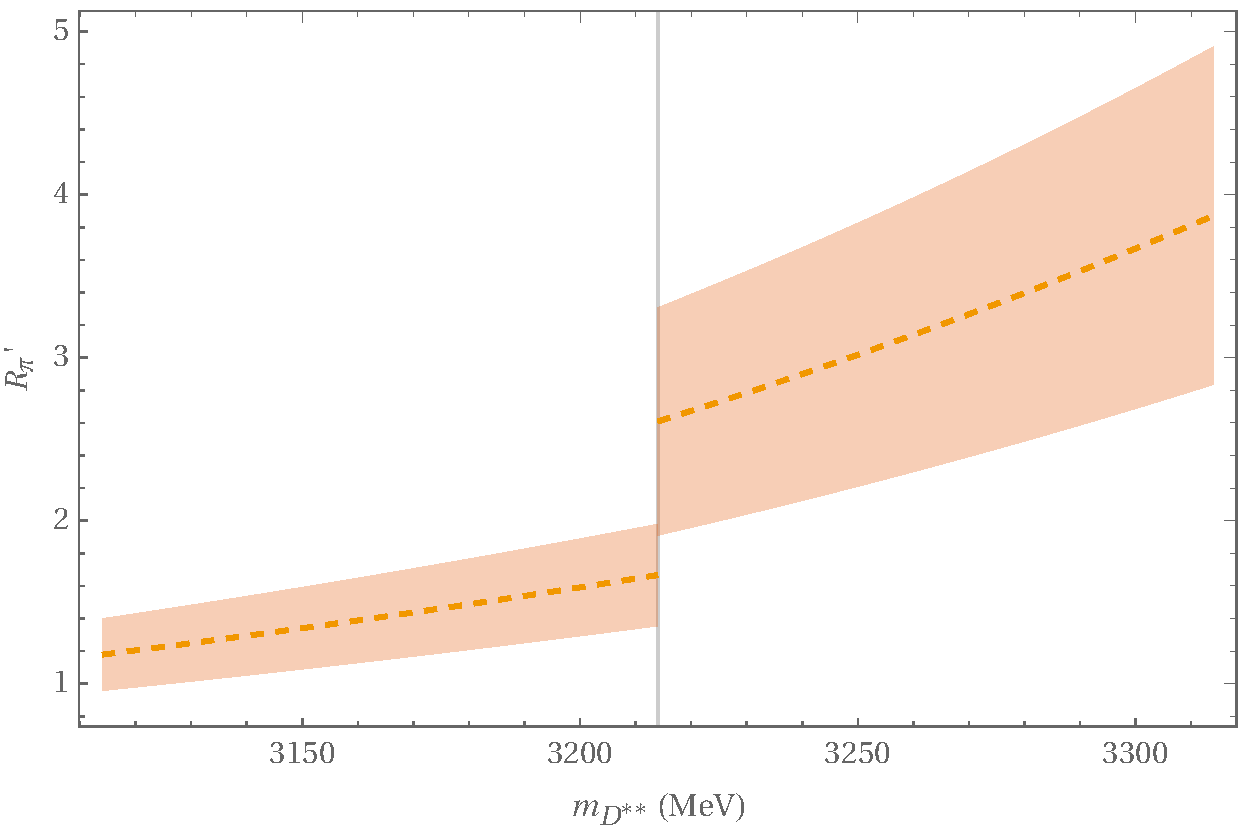
\includegraphics[width=\textwidth]{../figures/plot.pdf}
          \end{figure}
        \end{block}
      \end{column}
%      \begin{column}{0.5\textwidth}
%        The left-hand side refers to the case $D^{**}$ has $J^P=1^+$, the right-hand side to $J^P=3^+$.
%      \end{column}
    \end{columns}
\end{frame}

\subsection{Its Strange Partner}

\begin{frame}{What about its mass?}
  In (almost) all observed states the strange partner has a mass difference 
  of about $100 \ \text{\sfamily MeV}$. ← \emph{About the mass difference between 
  the strange and up/down quarks}
  \pause
  \begin{block}{An Educated Guess}
  \vspace{0pt}
    The strange partner of the $D^*_2(3000)$, namely the $D^{* \prime}_{s 2}$, should have mass $ \approx 3.3 \ \text{\sfamily GeV}$

    The value $m(D^{* \prime}_{s 2}) = 3313 \pm 62 \ \text{\sfamily MeV}$ is used.
  \end{block}
\end{frame}


\begin{frame}{Strange decays hierarchy}
  \begin{columns}
    \begin{column}[t]{0.5\textwidth}
      \begin{block}{Definitions}
        \vspace{0pt}
        \scriptsize
        \begin{align*}
          R_K &= \frac{\Gamma \left( D_{s 2}^{* +} \rightarrow D^{* 0} K^+ \right) + \Gamma \left( D_{s 2}^{* +} \rightarrow D^{* +} K_S \right)}{\Gamma \left( D_{s 2}^{* +} \rightarrow D^0 K^+ \right) + \Gamma \left( D_{s 2}^{* +} \rightarrow D^+ K_S \right)} \\
          R_\eta &= \frac{\Gamma \left( D_{s 2}^{* +} \rightarrow D_s^+ \eta \right)}{\Gamma \left( D_{s 2}^{* +} \rightarrow D^0 K^+ \right) + \Gamma \left( D_{s 2}^{* +} \rightarrow D^+ K_S \right)}  \\
          R^*_\eta &= \frac{\Gamma \left( D_{s 2}^{* +} \rightarrow D_s^{* +} \eta \right)}{\Gamma \left( D_{s 2}^{* +} \rightarrow D^0 K^+ \right) + \Gamma \left( D_{s 2}^{* +} \rightarrow D^+ K_S \right)} 
        \end{align*}
      \end{block}
    \end{column}
    \pause
    \begin{column}[t]{0.5\textwidth}
      \begin{block}{Calculated values}
        \vspace{0pt}
        \begin{table}
          \centering
          \begin{tabular}{*{3}{c}}
            \toprule
              & $\tilde{T}$ & $F$ \\
            \cmidrule{2-3}
            $R_K$ & $1.02 \pm 0.03$ & $0.39 \pm 0.02$ \\
            $R_\eta$ & $0.31 \pm 0.01$ & $0.29 \pm 0.01$ \\
            $R^*_\eta$ & $0.29 \pm 0.02$ & $0.10 \pm 0.01$ \\
            \bottomrule
          \end{tabular}
        \end{table}
      \end{block}
    \end{column}
  \end{columns}
  \pause
  \begin{block}{What does it mean?}
    \vspace{0pt}
    \begin{itemize}
      \item
        Case $D^*_2(3000)$ belongs to $\tilde{T}$: {} \alert{$R_K \gg \ R_\eta \approx R_\eta^*$}
      \item
        Case $D^*_2(3000)$ belongs to $F$: {} \alert{$R_K > R_\eta \gg R_\eta^*$}
    \end{itemize}
  \end{block}
\end{frame}

%  \begin{overlayarea}{\textwidth}{0.3\textheight}
%    \onslide<+->{
%      \begin{minipage}{0.5\textwidth}
%        \begin{block}{What does it mean?}
%          \vspace{0pt}
%          Case $D^*_2(3000)$ belongs to $\tilde{T}$
%          \begin{equation*}
%              R_K > R_\eta \gg R_\eta^*
%          \end{equation*}
%        \end{block}
%      \end{minipage}~
%    }
%    \only<+->{
%      \begin{minipage}{0.5\textwidth}
%        \begin{block}{What does it mean?}
%          \vspace{0pt}
%          Case $D^*_2(3000)$ belongs to $F$
%          \begin{equation*}
%            R_K \gg \ R_\eta \approx R_\eta^*
%          \end{equation*}
%        \end{block}
%      \end{minipage}
%    }
%  \end{overlayarea}

\section{Conclusions and Perspectives}

\begin{frame}{My thesis}
  \pause  
  \begin{block}{What has been done?}
    \begin{itemize}
      \item
        The whole observed spectrum of open-charm mesons has been presented
        and discussed.
      \item
        An original contribution aimed at the classification of the
        \(\left. D \right.^*_2(3000)\) has been presented.
    \end{itemize}
  \end{block}
  \vspace*{-\baselineskip}
  \begin{overlayarea}{\textwidth}{0.4\textheight}
    \only<2>{
      \begin{alertblock}{Summary of the Results for the Classification of the $D_2^*(3000)$}
        \vspace{10pt}
        \scriptsize
        \begin{columns}
          \begin{column}[t]{0.48\textwidth}
            Case $D_2^*(3000)$ belongs to the $F$ doublet
            \begin{itemize}
              \item 
                $R_\pi = 0.40 \pm 0.01$.
              \item 
                Spin partner: $D_3^*$, $J^P = 3^+$, $\approx 3.2\text{--}3.3 \ \text{GeV}$.
              \item 
                $R'_\pi = 3.60 \pm 1.60$.
              \item
                Strange partner: $R_K = 0.39 \pm 0.02 > R_\eta \gg R_\eta^*$.
            \end{itemize}
          \end{column}
          \begin{column}[t]{0.48\textwidth}
            Case $D_2^*(3000)$ belongs to the $\tilde{T}$ doublet
            \begin{itemize}
              \item
                $R_\pi = 1.06 \pm 0.03$.
              \item
                Spin partner: $\tilde{D}_1$, $J^P=1^+$, $\approx 3.1\text{--}3.2 \ \text{GeV}$.
              \item
                $R'_\pi = 1.50 \pm 0.60$.
              \item
                Strange partner: $R_K = 1.02 \pm 0.03 \gg \ R_\eta \approx R_\eta^*$.
            \end{itemize}
          \end{column}
        \end{columns}
      \end{alertblock}
    }
    \only<3>{
      \begin{block}{What could still be done?}
        \vspace{10pt}
        \begin{itemize}
          \item
            \emph{Within the same framework}: decays to excited $D$ mesons.
          \item
            \emph{Needing and extension of the framework}: decays with light
            vector mesons in the final state ($\rho$, $K^*$, $\omega$ and $\phi$).
        \end{itemize}
      \end{block}
    }
  \end{overlayarea}
\end{frame}

\begin{frame}{\textitalian{Qui finisce l'avventura}}
  \begin{figure}
    \center
    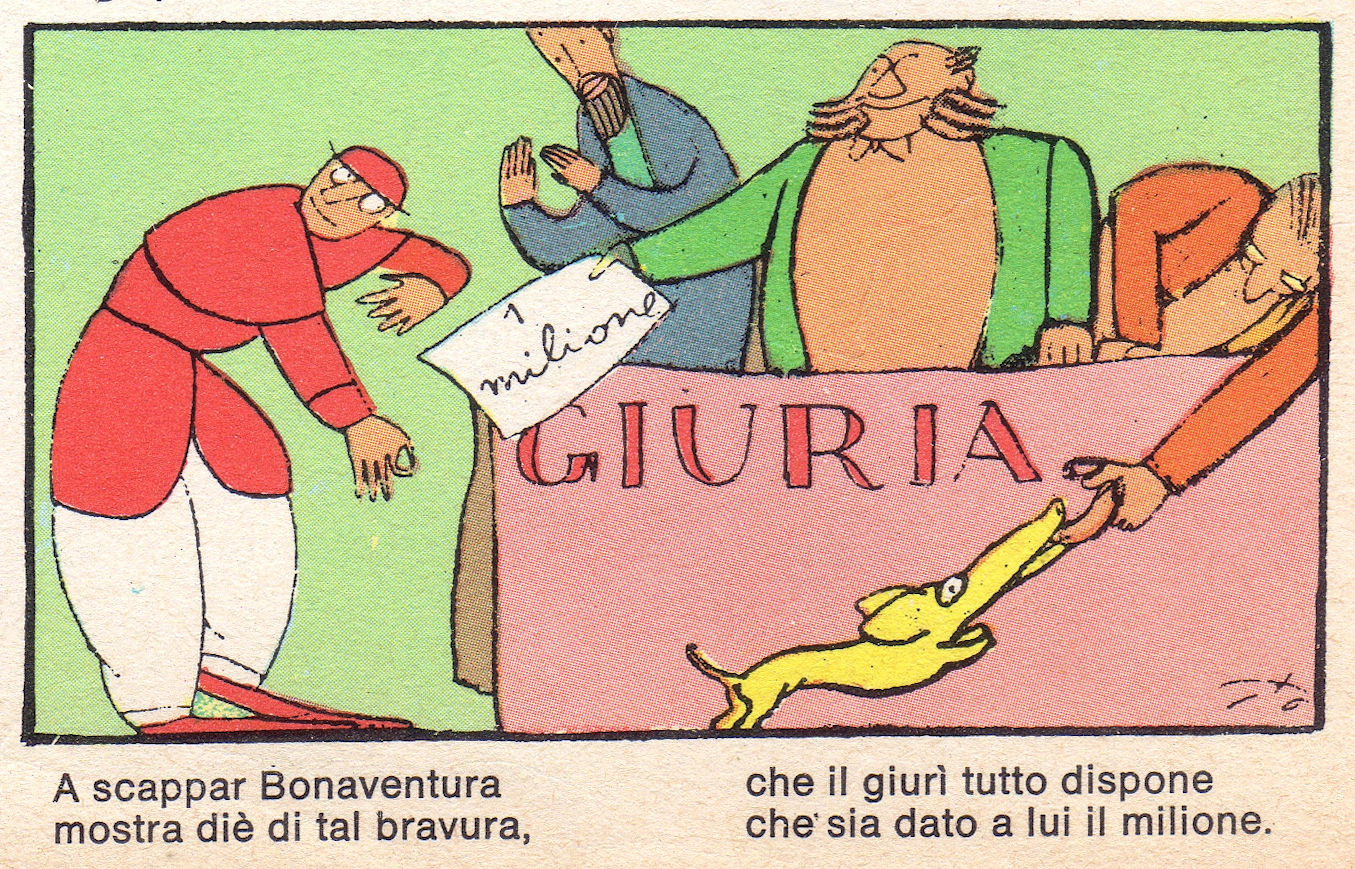
\includegraphics[width=0.8\textwidth]{../figures/bonaventura.jpg}
  \end{figure}
\end{frame}

\begin{frame}{Q\&A}
  \begin{quote}
    He who knows does not speak; he who speaks does not know.
  \end{quote}
  \begin{flushright}
    (Laozi, \emph{Tao Te Ching})
  \end{flushright}
\end{frame}

\end{document}

% vim: ft=tex nonumber wrap linebreak display+=lastline guifont=Inconsolata\ 20 spell spelllang=en_gb
